\chapter{The mpOTR Plugin}
\label{chapter:plugin}

In addition to the library we also extended the otr pidgin plugin's functionality.
It now uses the extended capabilities of libotr in order to provide private multi-party chatrooms.

Pidgin is an Instant Messaging (IM) client that is compatible with a wide range of IM protocols.
Since our protocol is protocol agnostic\footnote{This is not wholly true. Our implementation of mpOTR assumes that it can send messages of arbitrary length. This is not true in all IM protocols, IRC being one example.} pidgin users can readily chat securely with their existing contacts.

\section{The plugin workflow}

Allow us now to present in summary the workflow of the plugin.

This is what a pidgin chat conversation looks like when no mpOTR session is taking place.
Notice the mpOTR button on the lower right corner, similar to the OTR button.

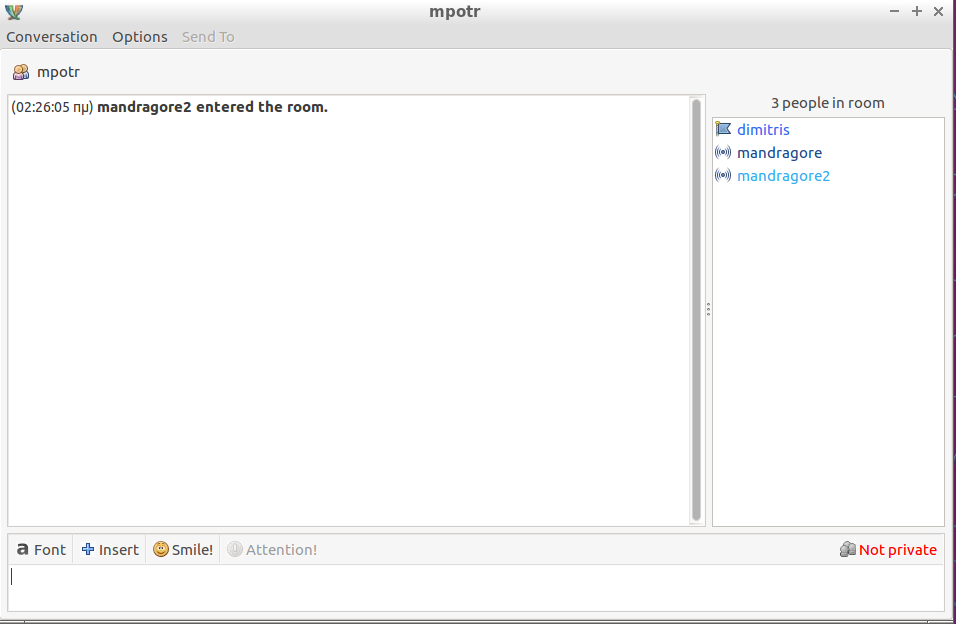
\includegraphics[scale=0.4]{not_started_unverified.png}

By clicking on the mpOTR button a user has the option to start a private conversation.
If he chooses to do so this is what he sees.

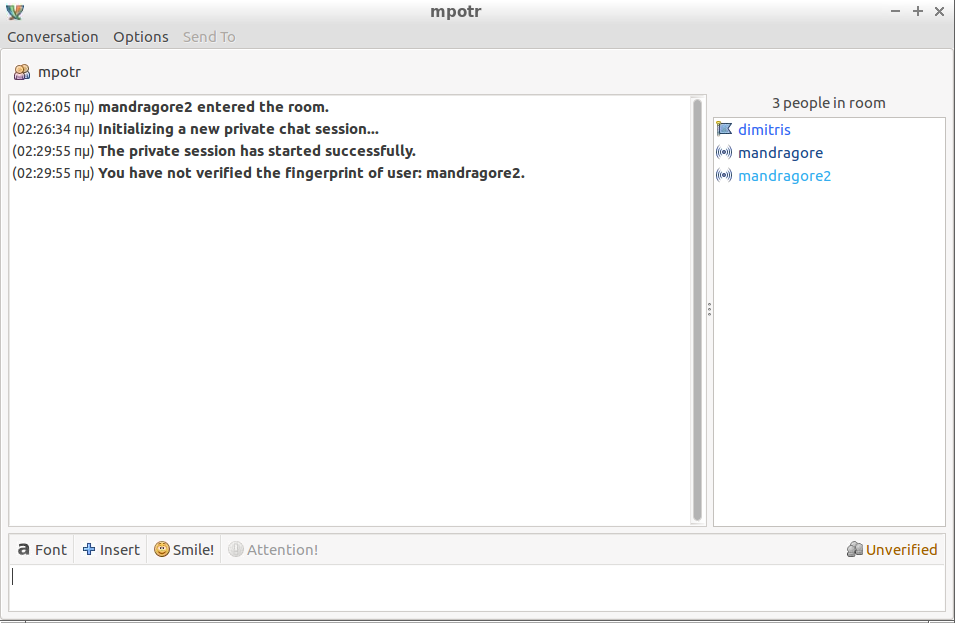
\includegraphics[scale=0.4]{started_unverified.png}

And when some texts are exchanged.

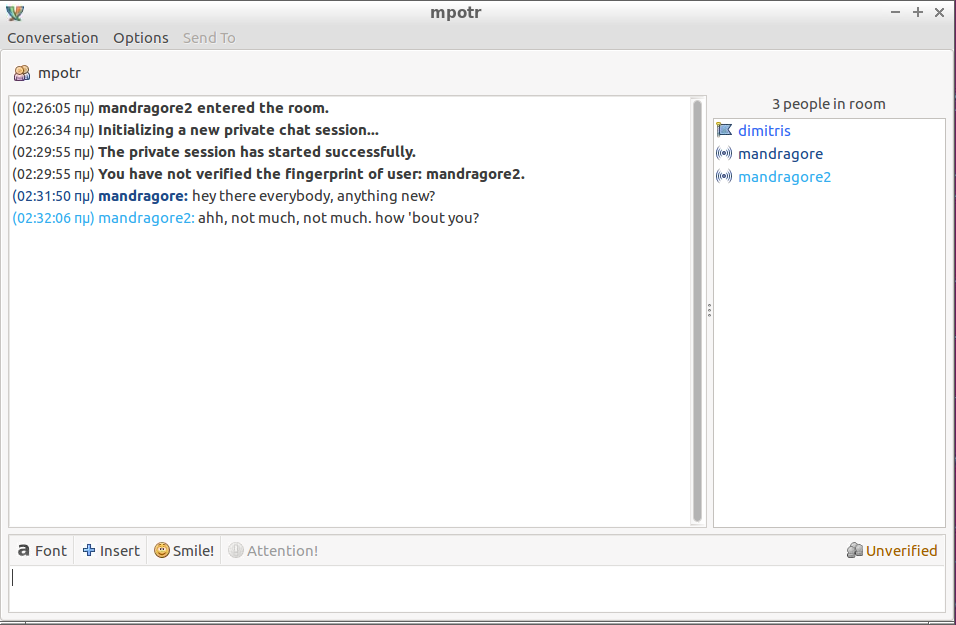
\includegraphics[scale=0.4]{talking_unverified.png}

However, our user (mandragore) hasn't verified another user (mandragore2).
This means that the conversation is unverified.
This is presented to the user in two ways.
First the mpOTR button has a yellow colour and states that the conversation is "Unverified".
And then, the message "You have not verified user: mandragore2".
This message will be displayed for every unverified user.

In order to verify the user mandragore2, our user clicks on the mpOTR button.
Notice how the "Start private conversation" option is now disabled.

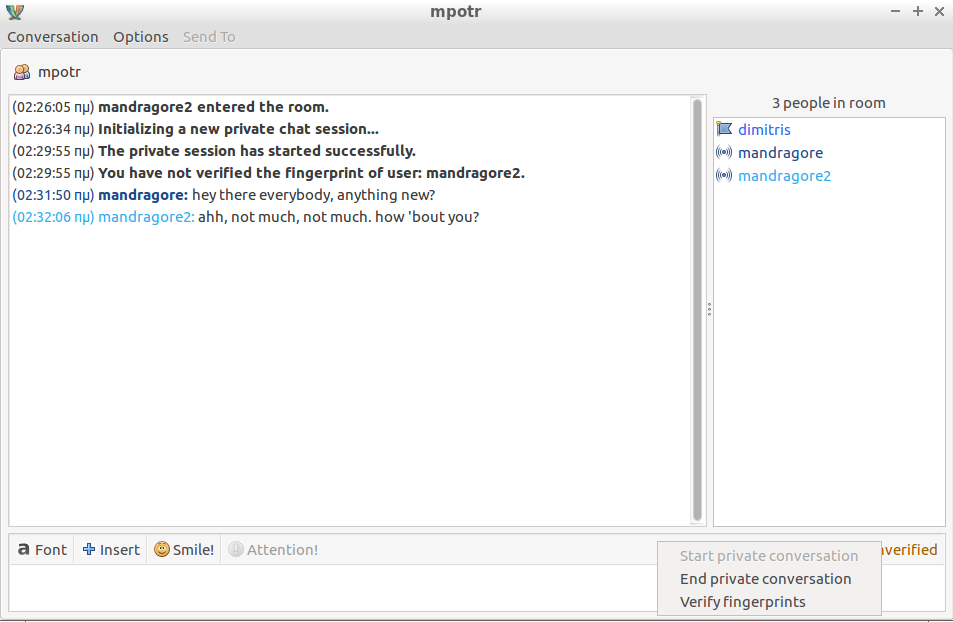
\includegraphics[scale=0.4]{click_mpotr_button_unverified.png}

If he clicks the "Verify fingerprints" option this window opens.

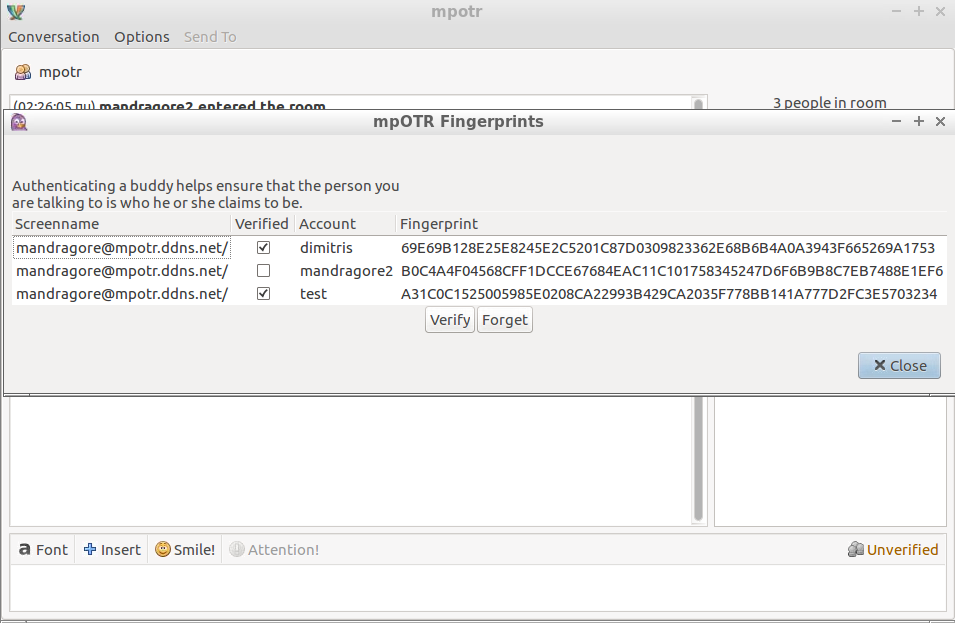
\includegraphics[scale=0.4]{verification_ui_opened_unverified.png}

In this window the user can click on the user he wants to verify and (after he checks the fingerprint) click on the "Verify" button.
The selected user will now be verified.

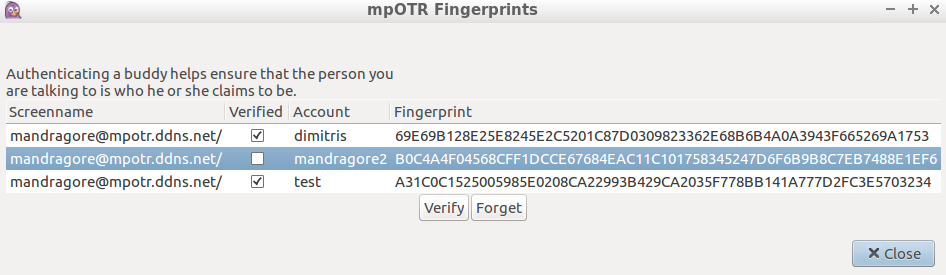
\includegraphics[scale=0.4]{verification_ui_selected_user_unverified.png}

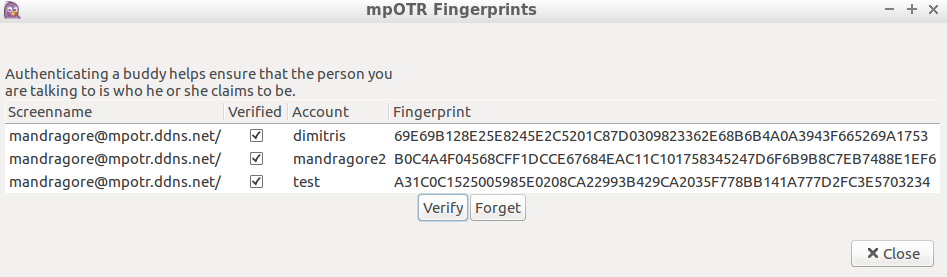
\includegraphics[scale=0.4]{user_verified_unverified.png}

To end the conversation the user clicks on the mpOTR button again and selects the "End private conversation" option.

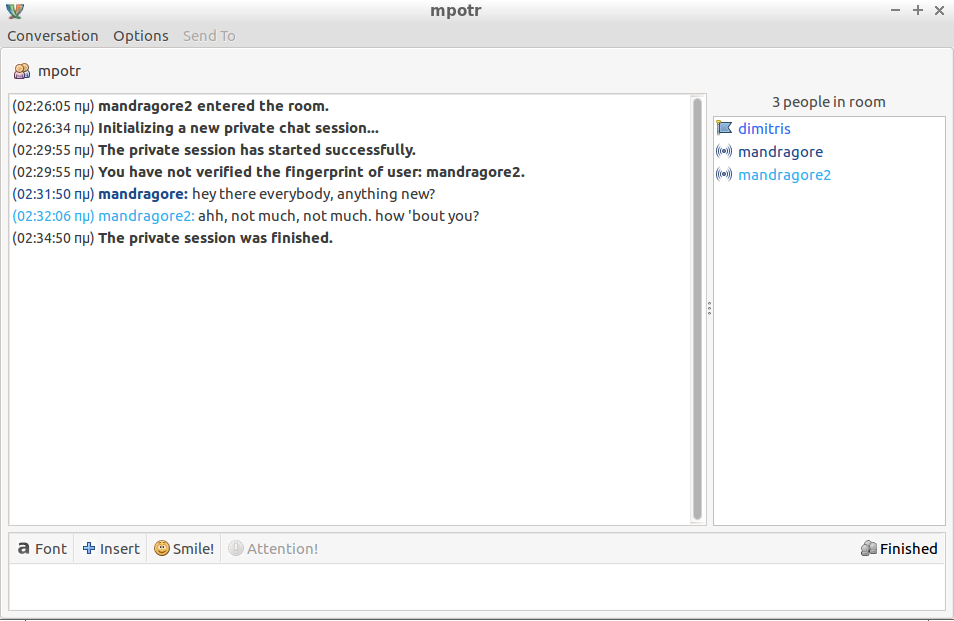
\includegraphics[scale=0.4]{finished_unverified.png}

Now if the user starts another private conversation the new session will be characterised as "Private".

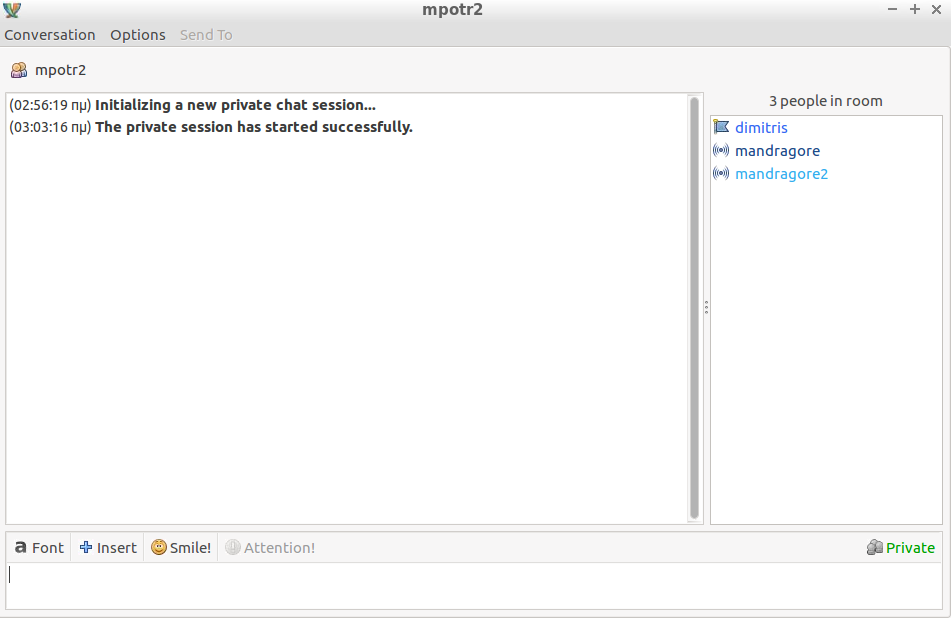
\includegraphics[scale=0.4]{started_verified.png}

